\documentclass[a4paper,11pt,twoside]{article}

\usepackage[T1]{fontenc}
\usepackage[utf8]{inputenc}

% packages
\usepackage[margin=2cm]{geometry}
\usepackage{amsmath}
\usepackage{amssymb}
\usepackage{upgreek}
\usepackage{fancyhdr}
\usepackage{caption}
\usepackage{emptypage}
\usepackage{tabularx}
\usepackage{parskip}
\usepackage{booktabs}
\usepackage[inline]{enumitem}
\usepackage{subfiles}
\usepackage{multicol}
\usepackage{placeins}
\usepackage{setspace}
\usepackage{xcolor}
\usepackage{boldline}
\usepackage{titlesec}

% Graphics
\usepackage[pdftex]{graphicx}
\usepackage{epsfig}
\usepackage[labelformat=simple]{subcaption}
\graphicspath{{Images/}}
\setkeys{Gin}{width=0.75\textwidth}
\renewcommand\thesubfigure{(\alph{subfigure})}
\captionsetup{width=0.9\textwidth}

% Font set (comment out to default to Computer Modern)
\usepackage{lmodern}
\renewcommand\familydefault{\sfdefault}
\allowdisplaybreaks

% Tikz defaults
\usepackage{tikz}
\usepackage{tikzpagenodes}
\usepackage{forest}
\usepackage{rotating}
\usepackage{subcaption}
\usetikzlibrary{arrows,patterns,calc,matrix,shapes,external}
\tikzset{point/.style={draw,fill,circle,inner sep=1pt}}

% Headers and footers
\usepackage{fancyhdr}
\pagestyle{fancy}
\fancyhf{}
\renewcommand{\sectionmark}[1]{\markright{#1}}

% Change \rightmark for online and print versions
\lhead{\includegraphics[width=3cm]{MMU_logo_1.png}}
\lfoot{Dr Jon Shiach}
\cfoot{\thepage}
\rfoot{Manchester Metropolitan University}
\fancyheadoffset{1cm}
\renewcommand{\headrulewidth}{0pt}
\setlength{\headheight}{2em}

% Shorthand commands
\newcommand{\vr}{\mathbf}
\newcommand{\unitvec}[1]{\hat{\mathbf{#1}}}
\newcommand{\floor}[1]{\left\lfloor #1 \right\rfloor}
\newcommand{\adj}{\operatorname{adj}}
\newcommand{\Span}{\operatorname{span}}
\newcommand{\REF}{Re\!f}
\newcommand{\ddx}{\dfrac{\mathrm{d}}{\mathrm{d}x}}

% Subsection headings
\titleformat{\section}
    {\normalfont\normalsize\bf}{Activity \thesection: }{0pt}{}

\title{Using Mathematics to Make and Stream Music: Activity Sheet}
\author{Dr Jon Shiach}
\date{}

\begin{document}

\maketitle
\thispagestyle{fancy}

\section{Calculating the co-ordinates of points on a circle}

Use the sine and cosine functions to calculate the co-ordinates of points on a circle with radius $r=3$ using angles $\theta = 0, \frac{\pi}{4}, \frac{2\pi}{4}, \frac{3\pi}{4} \ldots , 2\pi$. Remember to set your calculator to radians mode.

\begin{minipage}{0.5\textwidth}
    \centering
    \renewcommand{\arraystretch}{1.5}
    \begin{tabular}{V{2}>{\centering\arraybackslash}p{2cm}V{2}*{2}{>{\centering\arraybackslash}p{2cm}V{2}}}
         \hlineB{2}
         $\theta$ & $x = r\cos(\theta)$ & $y = r\sin(\theta)$ \\ \hlineB{2}  
         $0$ & $3$ & $0$ \\ \hlineB{2}
         $\frac{\pi}{4}$ & $2.12$ & $2.12$ \\ \hlineB{2}
         $\frac{2\pi}{4}$ & $0$ & $3$ \\ \hlineB{2}
         $\frac{3\pi}{4}$ & & \\ \hlineB{2}  
         $\pi$ & & \\ \hlineB{2}  
         $\frac{5\pi}{4}$ & & \\ \hlineB{2}  
         $\frac{6\pi}{4}$ & & \\ \hlineB{2}  
         $\frac{7\pi}{4}$ & & \\ \hlineB{2}  
         $2\pi$ & & \\ \hlineB{2}  
    \end{tabular}
\end{minipage}
\begin{minipage}{0.5\textwidth}
    \centering
    \begin{tikzpicture}
        \draw [-stealth'] (-3, 0) -- ++(6, 0) node [below] {$x$};
        \draw [-stealth'] (0, -3) -- ++(0, 6) node [left] {$y$};
        \foreach \i in {0, 45, ..., 315}{
            \draw [fill] (\i:2) circle (2pt);
        }
        \draw circle (2);
    \end{tikzpicture}
\end{minipage}

% \section{Plotting the sine wave}

% Calculate the $y$ co-ordinate of the points on a circle with radius $r = 1$ for the angles given in the table below. Plot the points with co-ordinates $(\theta, y)$ on the axes below and draw a smooth line through the points. Can you continue the curve up to $\theta = 720^\circ$?

% \begin{center}
%     \renewcommand{\arraystretch}{1.5}
%     \begin{tabular}{V{2}*{10}{>{\centering\arraybackslash}p{1.25cm}V{2}}}
%          \hlineB{2}
%          $\theta$ & $0^\circ$ & $45^\circ$ & $90^\circ$ & $135^\circ$ & $180^\circ$ & $225^\circ$ & $270^\circ$ & $315^\circ$ & $360^\circ$ \\ \hlineB{2}
%          $y$  & & & & & & & & & \\ \hlineB{2}
%     \end{tabular}
    
%     \begin{tikzpicture}
%         \draw [gray!20,step=0.3125] (0, -2.5) grid ++(11.25, 5);
%         \draw [gray!50,step=1.25] (0, -2.5) grid ++(11.25, 5);
%         \draw [-stealth'] (0, 0) -- ++(11.25, 0) node [below right] {$\theta$};
%         \draw [-stealth'] (0, -3) -- ++(0, 6) node [left] {$y$};
%         \foreach \i in {90, 180, ..., 720}{
%             \node [below] at ({\i / 72}, 0) {$\i$};
%         }
%         \foreach \i in {-1, -0.5, ..., 1}{
%             \node [left] at (0, {\i*2.5}) {$\i$};
%         }
%     \end{tikzpicture}
% \end{center}

\section{Changing the amplitude of a sine wave}

Complete the table for $y = 2\sin(\theta)$ and plot the curve on the axes below. How does multiplying $\sin(\theta)$ by $2$ change the shape of the sine wave?

\begin{center}
    \renewcommand{\arraystretch}{1.5}
    \begin{tabular}{V{2}*{10}{>{\centering\arraybackslash}p{1.25cm}V{2}}}
         \hlineB{2}
         $\theta$ & $0$ & $\frac{\pi}{4}$ & $\frac{\pi}{2}$ & $\frac{3\pi}{4}$ & $\pi$ & $\frac{5\pi}{4}$ & $\frac{3\pi}{2}$ & $\frac{7\pi}{4}$ & $2\pi$ \\ \hlineB{2}
         $y$  & $0$ & $1.4142$ & $2$ & & & & & & \\ \hlineB{2}
    \end{tabular}
    
    \begin{tikzpicture}
        \draw [gray!20,step=0.3125] (0, -2.5) grid ++(11.25, 5);
        \draw [gray!50,step=1.25] (0, -2.5) grid ++(11.25, 5);
        \draw [-stealth'] (0, 0) -- ++(11.25, 0) node [below right] {$\theta$};
        \draw [-stealth'] (0, -3) -- ++(0, 6) node [left] {$y$};
        \node [below] at (1.25, 0) {$\frac{\pi}{2}$};
        \node [below] at (2.5, 0) {$\pi$};
        \node [below] at (3.75, 0) {$\frac{3\pi}{2}$};
        \node [below] at (5, 0) {$2\pi$};
        \node [below] at (6.25, 0) {$\frac{5\pi}{2}$};
        \node [below] at (7.5, 0) {$3\pi$};
        \node [below] at (8.75, 0) {$\frac{7\pi}{2}$};
        \node [below] at (10, 0) {$4\pi$};
        \foreach \i in {-2, -1, ..., 2}{
            \node [left] at (0, {\i*1.25}) {$\i$};
        }
        \draw [domain=0:740,smooth,samples=100,gray] plot ({\x/72}, {1.25*sin(\x)}) node [right] {$y=\sin(\theta)$};
    \end{tikzpicture}
\end{center}

\section{Changing the frequency of a sine wave}

Complete the table for $y = \sin(2\theta)$ and plot the curve on the axes below. How does multiplying $\theta$ by $2$ change the shape of the sine wave?

\begin{center}
    \renewcommand{\arraystretch}{1.5}
    \begin{tabular}{V{2}*{10}{>{\centering\arraybackslash}p{1.25cm}V{2}}}
         \hlineB{2}
         $\theta$ & $0$ & $\frac{\pi}{4}$ & $\frac{\pi}{2}$ & $\frac{3\pi}{4}$ & $\pi$ & $\frac{5\pi}{4}$ & $\frac{3\pi}{2}$ & $\frac{7\pi}{4}$ & $2\pi$ \\ \hlineB{2}
         $y$  & $0$ & $1$ & $0$ & & & & & & \\ \hlineB{2}
    \end{tabular}
    
    \begin{tikzpicture}
        \draw [gray!20,step=0.3125] (0, -2.5) grid ++(11.25, 5);
        \draw [gray!50,step=1.25] (0, -2.5) grid ++(11.25, 5);
        \draw [-stealth'] (0, 0) -- ++(11.25, 0) node [below right] {$\theta$};
        \draw [-stealth'] (0, -3) -- ++(0, 6) node [left] {$y$};
        \node [below] at (1.25, 0) {$\frac{\pi}{2}$};
        \node [below] at (2.5, 0) {$\pi$};
        \node [below] at (3.75, 0) {$\frac{3\pi}{2}$};
        \node [below] at (5, 0) {$2\pi$};
        \node [below] at (6.25, 0) {$\frac{5\pi}{2}$};
        \node [below] at (7.5, 0) {$3\pi$};
        \node [below] at (8.75, 0) {$\frac{7\pi}{2}$};
        \node [below] at (10, 0) {$4\pi$};
        \foreach \i in {-1, -0.5, ..., 1}{
            \node [left] at (0, {\i*2.5}) {$\i$};
        }
        \draw [domain=0:740,smooth,samples=100,gray] plot ({\x/72}, {2.5*sin(\x)}) node [right] {$y=\sin(\theta)$};
    \end{tikzpicture}
\end{center}

\section{Changing the phase angle of a sine wave}

Complete the table for $y = \sin(\theta + \frac{\pi}{2})$ and plot the curve on the axes below. How does adding $\frac{\pi}{2}$ to $\theta$ change the shape of the sine wave?

\begin{center}
    \renewcommand{\arraystretch}{1.5}
    \begin{tabular}{V{2}*{10}{>{\centering\arraybackslash}p{1.25cm}V{2}}}
         \hlineB{2}
         $\theta$ & $0$ & $\frac{\pi}{4}$ & $\frac{\pi}{2}$ & $\frac{3\pi}{4}$ & $\pi$ & $\frac{5\pi}{4}$ & $\frac{3\pi}{2}$ & $\frac{7\pi}{4}$ & $2\pi$ \\ \hlineB{2}
         $y$  & $1$ & $0.7071$ & $0$ & & & & & & \\ \hlineB{2}
    \end{tabular}
    
    \begin{tikzpicture}
        \draw [gray!20,step=0.3125] (0, -2.5) grid ++(11.25, 5);
        \draw [gray!50,step=1.25] (0, -2.5) grid ++(11.25, 5);
        \draw [-stealth'] (0, 0) -- ++(11.25, 0) node [below right] {$\theta$};
        \draw [-stealth'] (0, -3) -- ++(0, 6) node [left] {$y$};
        \node [below] at (1.25, 0) {$\frac{\pi}{2}$};
        \node [below] at (2.5, 0) {$\pi$};
        \node [below] at (3.75, 0) {$\frac{3\pi}{2}$};
        \node [below] at (5, 0) {$2\pi$};
        \node [below] at (6.25, 0) {$\frac{5\pi}{2}$};
        \node [below] at (7.5, 0) {$3\pi$};
        \node [below] at (8.75, 0) {$\frac{7\pi}{2}$};
        \node [below] at (10, 0) {$4\pi$};
        \foreach \i in {-1, -0.5, ..., 1}{
            \node [left] at (0, {\i*2.5}) {$\i$};
        }
        \draw [domain=0:740,smooth,samples=100,gray] plot ({\x/72}, {2.5*sin(\x)}) node [right] {$y=\sin(\theta)$};
    \end{tikzpicture}
\end{center}

\newpage
\section{Adding sine waves together}

Complete the table for $y = 2\sin(\theta) + \sin(2\theta) + \sin(\theta + \frac{\pi}{2})$ and plot the curve on the axes below. You can use your calculations from the previous activities to help you with this.

\begin{center}
    \renewcommand{\arraystretch}{1.5}
    \begin{tabular}{V{2}*{10}{>{\centering\arraybackslash}p{1.25cm}V{2}}}
         \hlineB{2}
         $\theta$ & $0$ & $\frac{\pi}{4}$ & $\frac{\pi}{2}$ & $\frac{3\pi}{4}$ & $\pi$ & $\frac{5\pi}{4}$ & $\frac{3\pi}{2}$ & $\frac{7\pi}{4}$ & $2\pi$ \\ \hlineB{2}
         $y$  & $1$ & $3.121$ & $2$ & & & & & & \\ \hlineB{2}
    \end{tabular}
    
    \begin{tikzpicture}
        \draw [gray!20,step=0.3125] (0, -3) grid ++(11.25, 7.5);
        \draw [gray!50,step=1.25] (0, -3) grid ++(11.25, 7.5);
        \draw [-stealth'] (0, 0) -- ++(11.25, 0) node [below right] {$\theta$};
        \draw [-stealth'] (0, -3.5) -- ++(0, 8.5) node [left] {$y$};
        \node [below] at (1.25, 0) {$\frac{\pi}{2}$};
        \node [below] at (2.5, 0) {$\pi$};
        \node [below] at (3.75, 0) {$\frac{3\pi}{2}$};
        \node [below] at (5, 0) {$2\pi$};
        \node [below] at (6.25, 0) {$\frac{5\pi}{2}$};
        \node [below] at (7.5, 0) {$3\pi$};
        \node [below] at (8.75, 0) {$\frac{7\pi}{2}$};
        \node [below] at (10, 0) {$4\pi$};
        \foreach \i in {-2, -1, ..., 3}{
            \node [left] at (0, {\i*1.25}) {$\i$};
        }
        % \draw [domain=0:740,smooth,samples=100,gray] plot ({\x/72}, {2.5 * sin(\x) + 1.25 * sin(2 * \x) + 1.25 * sin(\x + 90});
    \end{tikzpicture}
\end{center}

\end{document}